\section{Основные понятия теории вероятностей}
\subsection{Предмет статистической радиофизики}

Статистическая радиофизика изучает случайные явления в радиофизике.
Статистическое описание является наиболее подходящим для многих электромагнитных
явлений. Статистическая радиофизика изучает случайные процессы на всех этапах
радиосвязи.

Статистическая радиофизика использует методы радиофизики, статистической физики
и теории вероятностей и работает с информационными характеристиками (дисперсией,
корелляцией, \ldots).

Под сообщением понимаются любые данные или сведения, подлежащие передаче. По
своей природе сообщения делятся на механические, тепловые, электромагнитные и
т.д. Сообщения неэлектрической природы часто преобразуют в электрический сигнал
при помощи преобразователей. При необходимости, электрический сигнал для
передачи преобразуют в радиосигнал.

При преобразовании, передаче, распространении и приёме сигнал подвергается
искажениям. Они обуславливаются:
\begin{enumerate}
    \item внешними и внутренними помехами;
    \item распространением сигнала через турбулентную среду;
    \item техническим несовершенством устройств.
\end{enumerate}
Любые нежелательные возмущения, накладывающиеся на сигнал, называются шумом.

\subsection{Вероятность}

Основное понятие радиофизики -- случайная величина. Случайная величина -- это
форма представления заранее не предсказуемых результатов опыта. Для описания
случайных величин в математике вводится понятие вероятности.

Вероятность события \( A \) есть отношение числа опытов, в которых происходило
это событие, к общему числу опытов при стремлении числа опытов к бесконечности:
\[
    P(A) = \lim_{N\to\infty}\frac{N_A}{N}.
\]

Если событие не может произойти ни в одном опыте, то вероятность такого события
равна нулю, а событие называется невозможным.

Если же событие происходит в каждом опыте, то его вероятность равна единице, а
само событие называется достоверным.

Если два события никогда не происходят вместе, то такие события называются
несовместимыми.

Событие, представляющее собой множество вероятных исходов составляет группу
событий. Группа называется полной, если в результате опыта произойдет одно из
событий этой группы.

Два события, образующие полную группу, называются противоположными, если они
несовместимы.

Если всякий раз, когда происходит событие \( A \), происходит событие \( B \),
то говорят, что \( A \) влечет за собой \( B \): \( A \subset B \). Если
\( A \subset B \) и \( B \subset A \), то \( A = B \) и такие события называют
равносильными или эквивалентными.

Событие \( A \) называется статистически зависимым от события \( B \), если
\( P(A) \) зависит от того, осуществилось ли событие \( B \) или нет. В случае
статистической зависимости можно ввести условную вероятность \( P(A|B) \)
события \( A \) при осуществлении события \( B \). Безусловные вероятности
называются априорными, а условные -- апостериорными.

Произведением событий называется такое событие, которое происходит, когда
одновременно происходят все эти события:
\[
    P(AB) = P(A) \cdot P(B|A) = P(B) \cdot P(A|B).
\]

Суммой событий называется событие, которое происходит тогда и только тогда,
когда происходит хотя бы одно из этих событий:
\[
    P(A+B) = P(A) + P(B) - P(AB).
\]

Если события несовместимы и образуют полную группу, то
\[
    P\left(\sum A_i\right) = \sum P(A_i) = 1.
\]
Это условие называется условием нормировки.

Пусть несовместимые события \( B \) и \( C \) входят в полную группу, а \( A \)
может произойти только при наступлении этих двух событий, тогда
\[
    P(A) = P(AB) + P(AC) = P(B) \cdot P(A|B) + P(C) \cdot P(A|C).
\]
Эта формула называется формулой полной вероятности.
\[
    P(B|A) = \frac{P(AB)}{P(A)} = \frac{P(B) \cdot P(A|B)}
    {P(B) \cdot P(A|B) + P(C) \cdot P(A|C)} \text{ -- формула Байеса.}
\]

В технике используются системы, состоящие из нескольких элементов. Надежностью
системы называют вероятность того, что система будет работать без отказа в
течение установленного промежутка времени. Пусть система состоит из двух
элементов, причем надежность первого \( P_1 \), а второго \( P_2 \). Тогда
надежность при последовательном соединении равна \( P_1P_2 \),  а при
параллельном~--\\ \( 1 - (1 - P_1)(1 - P_2) = P_1 + P_2 - P_1P_2 \).

\subsection{Функция распределения случайной величины}

Соотношение, устанавливающее связь между возможным значением случайной величины
и её вероятностью, называется функцией распределения.

Пусть случайная величина \( X \) каким-либо образом распределена на
\( \mathbb{R} \). Тогда \( F(x) = P(X \le x) \) называется (интегральной)
функцией распределения величины \( X \). Эта функция обладает следующими
свойствами:
\begin{itemize}
    \item для дискретной величины \( \ds F(x) = \sum_{X_i \le x}P(X_i) \);
    \item для непрерывной величины \( \ds F(x) = \int_{-\infty}^x w(\xi)d\xi \);
    \item \( F(-\infty) = 0 \);
    \item \( F(+\infty) = 1 \);
    \item \( F(x) \) -- монотонно неубывающая функция;
    \item \( P(x_1 < X < x_2) = F(x_2) - F(x_1) \);
    \item для непрерывно распределенной величины является гладкой всюду
        непрерывной функцией.
\end{itemize}
В случае непрерывной величины функция
\[
    w(x) = \der{F(x)}{x}
\]
называется плотностью распределения. Она обладает рядом свойств:
\begin{itemize}
    \item \( \ds \int_{-\infty}^{+\infty} w(\xi) d\xi = 1 \);
    \item \( \forall x\ w(x) \ge 0 \);
    \item для дискретной величины
        \( \ds w(x) = \sum_i P(X_i) \cdot \delta(x - X_i) \).
\end{itemize}

Для любой функции случайной величины можно ввести понятие среднего значения
\[
    \average{f(x)} = \int_{-\infty}^{+\infty}f(x)w(x)dx,
\]
переходящее для дискретной величины в
\[
    \average{f(x)} = \sum_i P(X_i)f(X_i).
\]

\subsection{Моменты случайной величины}

Момент \( m_n \) \( n \)-го порядка определяется выражением
\[
    m_n(X) = \average{X^n} = \int_{-\infty}^{+\infty} x^n w(x) dx.
\]
\( m_1 \) называется средним значением или математическим ожиданием.

Центральный момент \( \mu_n \) \( n \)-го порядка определяется выражением
\[
    \mu_n(X) = \average{\left(X - \average{X}\right)^n}.
\]
\( \mu_2 = \sigma^2 \) называется дисперсией, а \( \sigma \) --
среднеквадратичным отклонением.

\subsection{Совместное распределение}
Для двух случайных величин \( X \) и \( Y \) можно ввести двухмерную функцию
распределения \( F(x,y) = P(X \le x, Y \le y) \). Эта функция обладает всеми
свойствами одномерной функции распределения. Кроме того,
\( F(x, +\infty) = F_x(x) \). Для непрерывно распределенных величин можно ввести
плотность распределения
\[
    w(x,y) = \pcder{F(x,y)}{x}{y} \ge 0.
\]
Тогда
\[
    F(x, y) = \int_{-\infty}^x\int_{-\infty}^y w(\xi,\eta)d\xi d\eta,\quad
    F_x(x) = \int_{-\infty}^x\int_{-\infty}^{+\infty} w(\xi,\eta)d\xi d\eta.
\]

Для независимых событий
\( F(x,y) = F_x(x) \cdot F_y(y), w(x,y) = w_x(x) \cdot w_y(y) \).

Для зависимых можно ввести условную функцию распределения
\begin{gather*}
    F(y|x) = \lim_{\xi \to x} P(\xi < X \le x, Y \le y),\quad
    w(y|x) = \pder{F(y|x)}{y} \ge 0,\\
    w_y(y) = \int_{-\infty}^{+\infty} w(y|x) w_x(x) dx.
\end{gather*}

Смешанный момент
\[
    m_{kn} = \int_{-\infty}^{+\infty}\int_{-\infty}^{+\infty}x^ky^nw(x,y)dxdy,
\]
центральный момент
\[
    \mu_{kn} = \int_{-\infty}^{+\infty}\int_{-\infty}^{+\infty}
        \left(x-\average{X}\right)^k
        \left(y-\average{Y}\right)^n w(x,y)dxdy.
\]
Очевидно, что
\[
    \average{X} = m_{10},\ \average{Y} = m_{01},\ \sigma_x^2 = \mu_{20},
    \ \sigma_y^2 = \mu_{02}.
\]
\( B = m_{11} \) называется ковариацией, а
\[
    r = \frac{B}{\sigma_x\sigma_y}
\]
кореляционным моментом. Для независимых случайных величин оба этих числа равны
нулю. В этом случае случайные величины называются ортогональными.

\subsection{Задачи}
\begin{enumerate}
    \item По линии связи в случайном порядке передаются 30 знаков русского
        алфавита. Найти вероятность того, что на ленте появится
        последовательность букв, образующая слово ``радио'' при передачи 5
        знаков.

        5 букв из 30 с учётом их порядка можно выбрать
        \( A_{30}^{5} = 30\cdot29\cdot28\cdot27\cdot26 \) способами.
        Следовательно, вероятность того, что эти 5 букв составят слово ``радио''
        равна
        \[
            \frac{1}{30\cdot29\cdot28\cdot27\cdot26} = 5.8\cdot10^{-8}.
        \]
    \item В партии из 10 радиоламп имеются 4 нестандартные. Для проверки
        выбирают наугад 5 радиоламп. Определите вероятность того, что среди них
        будут 2 нестандартные.

        5 ламп из 10 можно выбрать \( C_{10}^5 \) способами. При этом, среди них
        должно оказаться 2 нестандартные, которые можно выбрать \( C_4^2 \)
        способами, и 3 стандартные, которые выбираются \( C_6^3 \) способами.
        Искомая вероятность определяется формулой
        \[
            \frac{C_6^3 \cdot C_4^2}{C_{10}^5} = \frac{10}{21}.
        \]
    \item В любой момент интервала времени \( T \) равновозможно поступление
        двух независимых сигналов. Приёмник будет перегружен, если разность
        между моментами поступления сигнала будет меньше \( \tau \). Определить
        вероятность перегруза.
        \begin{figure}[h]
        \begin{center}
            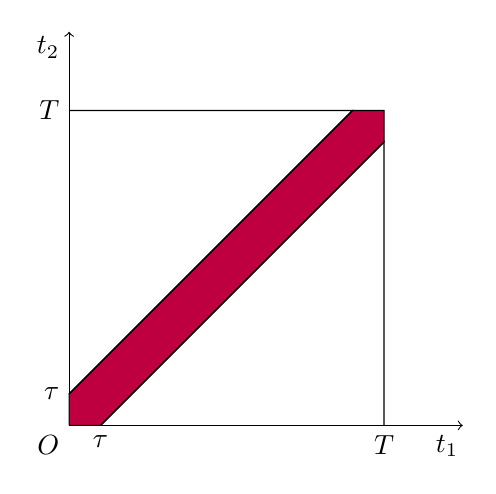
\begin{tikzpicture}
                \draw [<->] (0, 5) -- (0, 0) -- (5, 0);
                \node [below] at (4.8, 0) {\( t_1 \)};
                \node [left] at (0, 4.8) {\( t_2 \)};
                \draw [fill=purple] (0, 0) -- (0.4, 0) -- (4, 3.6) -- (4, 4) --
                    (3.6, 4) -- (0, 0.4) -- (0, 0);
                \draw (0.4, 0) -- (4, 3.6) -- (4, 0);
                \draw (0, 0.4) -- (3.6, 4) -- (0, 4);
                \node [below] at (0.4, 0) {\( \tau \)};
                \node [below] at (4, 0) {\( T \)};
                \node [below left] at (0, 0) {\( O \)};
                \node [left] at (0, 0.4) {\( \tau \)};
                \node [left] at (0, 4) {\( T \)};
            \end{tikzpicture}
        \end{center}
        \end{figure}

        Воспользуемся геометрической вероятностью. Для этого изобразим все
        возможные времена приёма сигналов на плоскости. Тогда все возможные
        события образуют квадрат со стороной \( T \). Область, соответствующая
        перегрузке определяется условием \( |t_1 - t_2| \le \tau \) и
        представляет из себя закрашенный шестиугольник. Тогда вероятность
        перегрузки определяется выражением
        \[
            \frac{T^2 - (T-\tau)^2}{T^2} =
            \frac{\tau}{T}\left(2 - \frac{\tau}{T}\right).
        \]

\end{enumerate}
